\subsection{Personalizacion}
So far we have seen different parameters to consider the relevant data at a general level, in this section, we
We will focus on a personal level.
Each user is unique as well as their personal situation, so we will have to find a way to get the data
adapt to users. Offer you information not only relevant at a general level but at a particular level.
Posing that we need to be told the data in my case, by the place where I live, by
my health, family situation, something that characterizes us can help us.

In many cases, we will not be able to fully customize it, but we can look for common points in subgroups of
users, from this point you have to study the different cases that can be given and make a selection of those that are
more common.


\subsubsection{How to solve it} 

Study in what way the data will help the user or the subgroups and from this point, make it more specific, in this way
  we will go from obtaining relevant data in a general way to be relevant in a personal way. You have to think about the
  user, not in the users and find the way to find the results that are specifically adapted to him.
 \subsubsection{How we solve it. Aire Guru} 
 We are all interested in the pollution that surrounds us, since it is important for our health, for this reason, the tool
 Aire Guru has specialized in this area. For those people who are especially sensitive to the pollution of the
 Air, Air Guru shows the air pollution with respect to the six most common medical conditions that
 they are affected by some contaminant.
 

\begin{figure}[ht]
    \centering
   \subfigure[EPOC]
    {\includegraphics[width=3.5cm  ]{filter_epoc}}
    \hfill
    \subfigure [Asthma]
       { 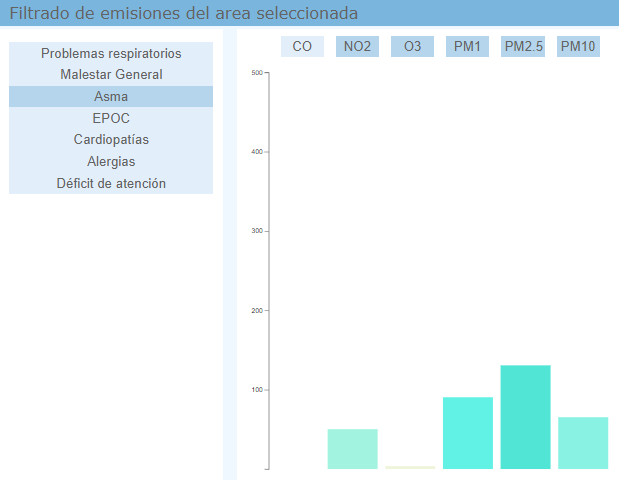
\includegraphics[width=3.5cm]{filter_asthma}}
    \hfill
     \subfigure[Allergies]
     {   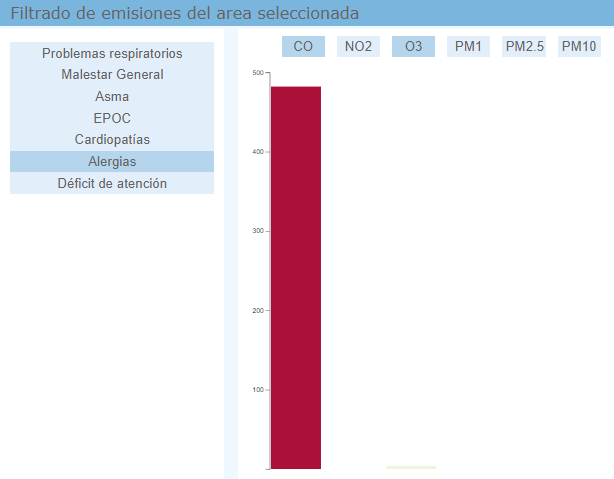
\includegraphics[width=3.5cm]{filter_allergies}}
  
  \caption{Medical Condition Filter}
    \end{figure}
    As we see, in each of the cases, for each medical condition, it shows a subset of pollutants,
      those that most influence each medical condition.
    
      Another customization feature is the representation of the exposure to pollution for each user.
      As we can see in figure X. Personal Records, the user is able to see the pollution that has surrounded him specifically
      to him over time.

 
\elsparagraph{Evaluation}  
\begin{itemize}
   \done The user has specialized functionalities
        \crossed The filtering function of the medical condition is not self-selected, this is because the functionality
        It is available to all users. It could be implemented so that the map would show the AQI with respect to the
        contaminants that the user has preselected, but this can de-virtualize the information if it is not
        clearly indicates to the user that the map does not take into account all relevant contaminants.
\end{itemize}
 \newpage